\mcsubsection{Definition and early developments}

In the general context of QCD studies, the term ``hadronization'' has
been used with somewhat different meanings. 
In the present context it refers to the specific
model used in an event generator for the transition from the partonic
``final'' state to a complete representation of the actual hadronic
final state.  We should emphasize that this is a transition for which we
still have only models, albeit inspired by QCD, because the only
available rigorous approach to non-perturbative hadronic phenomena, lattice
QCD, is formulated in Euclidean space-time and therefore cannot deal
with inherently Minkowskian processes like the time-evolution of
partons into hadrons.

Other ``hadronization'' meanings exist. When quantities that
are calculable within perturbative QCD, for example hadronic event
shapes in $e^+e^-$ annihilation, are compared with experimental data,
there are discrepancies that are commonly ascribed to ``hadronization
corrections''.  They are often estimated and corrected for by comparing
the hadron-level prediction of an event generator with a parton-level
result computed at the end of parton showering.\footnote{We strongly
  deprecate the correction of experimental data to ``parton level''
  by this method. See \SecRef{sec:phys-phil-behind} for discussion of
  this point.}  However, such a
parton-level quantity is not really comparable to the result of a
perturbative calculation, certainly not at fixed order, nor even when
resummed to all orders, as the shower result depends on the scale and
details of the cutoff that terminates it.  The origin of the
discrepancies is instead generic non-perturbative contributions
that do not depend on the detailed mechanism of hadron
formation.  They can be parameterized as power-suppressed terms
related to the so-called infrared renormalon ambiguity of the perturbation
series~\cite{Webber:1994cp,Korchemsky:1994is,Dokshitzer:1995zt,Dokshitzer:1995qm}.

Another use of the term hadronization is to describe the
parameterization of single-particle distributions from hard processes
in terms of fragmentation functions -- for recent reviews
see~\cite{Amsler:2008zzb,Albino:2008gy}.
This is analogous to the parameterization of PDFs for incoming hadrons,
and indeed similar factorization properties allow the scale dependence
of the distributions to be predicted once they have been fitted at
some scale, for example in $e^+e^-$ annihilation.  However once again
such analyses do not illuminate the mechanism of hadron formation.

The earliest models for hadronic final states were based 
on isotropic or longitudinal phase space. On their own, these are 
mainly of interest at very low energies, and are not discussed 
further. The first model that points the way to current approaches 
is the Artru--Mennessier one \cite{Artru:1974hr}, which manages to 
pioneer both string and cluster concepts. The code had a 
number of limitations, however, and never had a practical impact.

In contrast, the Field--Feynman model \cite{Field:1977fa} 
a few years later kickstarted the whole field of hadronization
studies by Monte Carlo simulation. It introduced an iterative 
recipe for the construction of realistic jets. By considering each
outgoing parton separately, it became possible to write 
``independent fragmentation'' generators for $e^+e^-$ physics 
\cite{Hoyer:1979ta,Ali:1979em}.\footnote{We note here that historically the terms
  ``fragmentation'' and ``hadronization'' have been used
  interchangeably, and we follow that usage in this Section, although in other
  contexts fragmentation can refer to the whole process of parton
  showering plus hadron formation.} These models soon became outdated
since the independent fragmentation framework is not Lorentz invariant, 
is not safe under collinear emissions of partons, and also suffers 
from other deficiencies \cite{Sjostrand:1984iy}.

The two main hadronization classes in current use are the string 
and cluster ones. These are described in the following. The main 
difference is that the former transforms partonic systems
directly into hadrons, while the latter employs an intermediate 
stage of cluster objects, with a typical mass scale of a few GeV.

\mcsubsection{String model}
\label{sec:string-model}

An early string fragmentation model is that of Artru and Mennessier, 
introduced above. The most sophisticated and well-known string 
model is the Lund one, however. Its development began in 1977,  
followed by the first primitive Monte Carlo implementation in 1978. 
The core framework was complete by 1983 \cite{Andersson:1983ia,%
Andersson:1998tv}. Thereafter many different additions and 
alternatives have been studied, but only 
a few of them are available in the standard implementation in the 
\pythia event generator \cite{Sjostrand:2006za,Sjostrand:2007gs}.
It is this core Lund string framework that is presented here.  

\begin{figure}
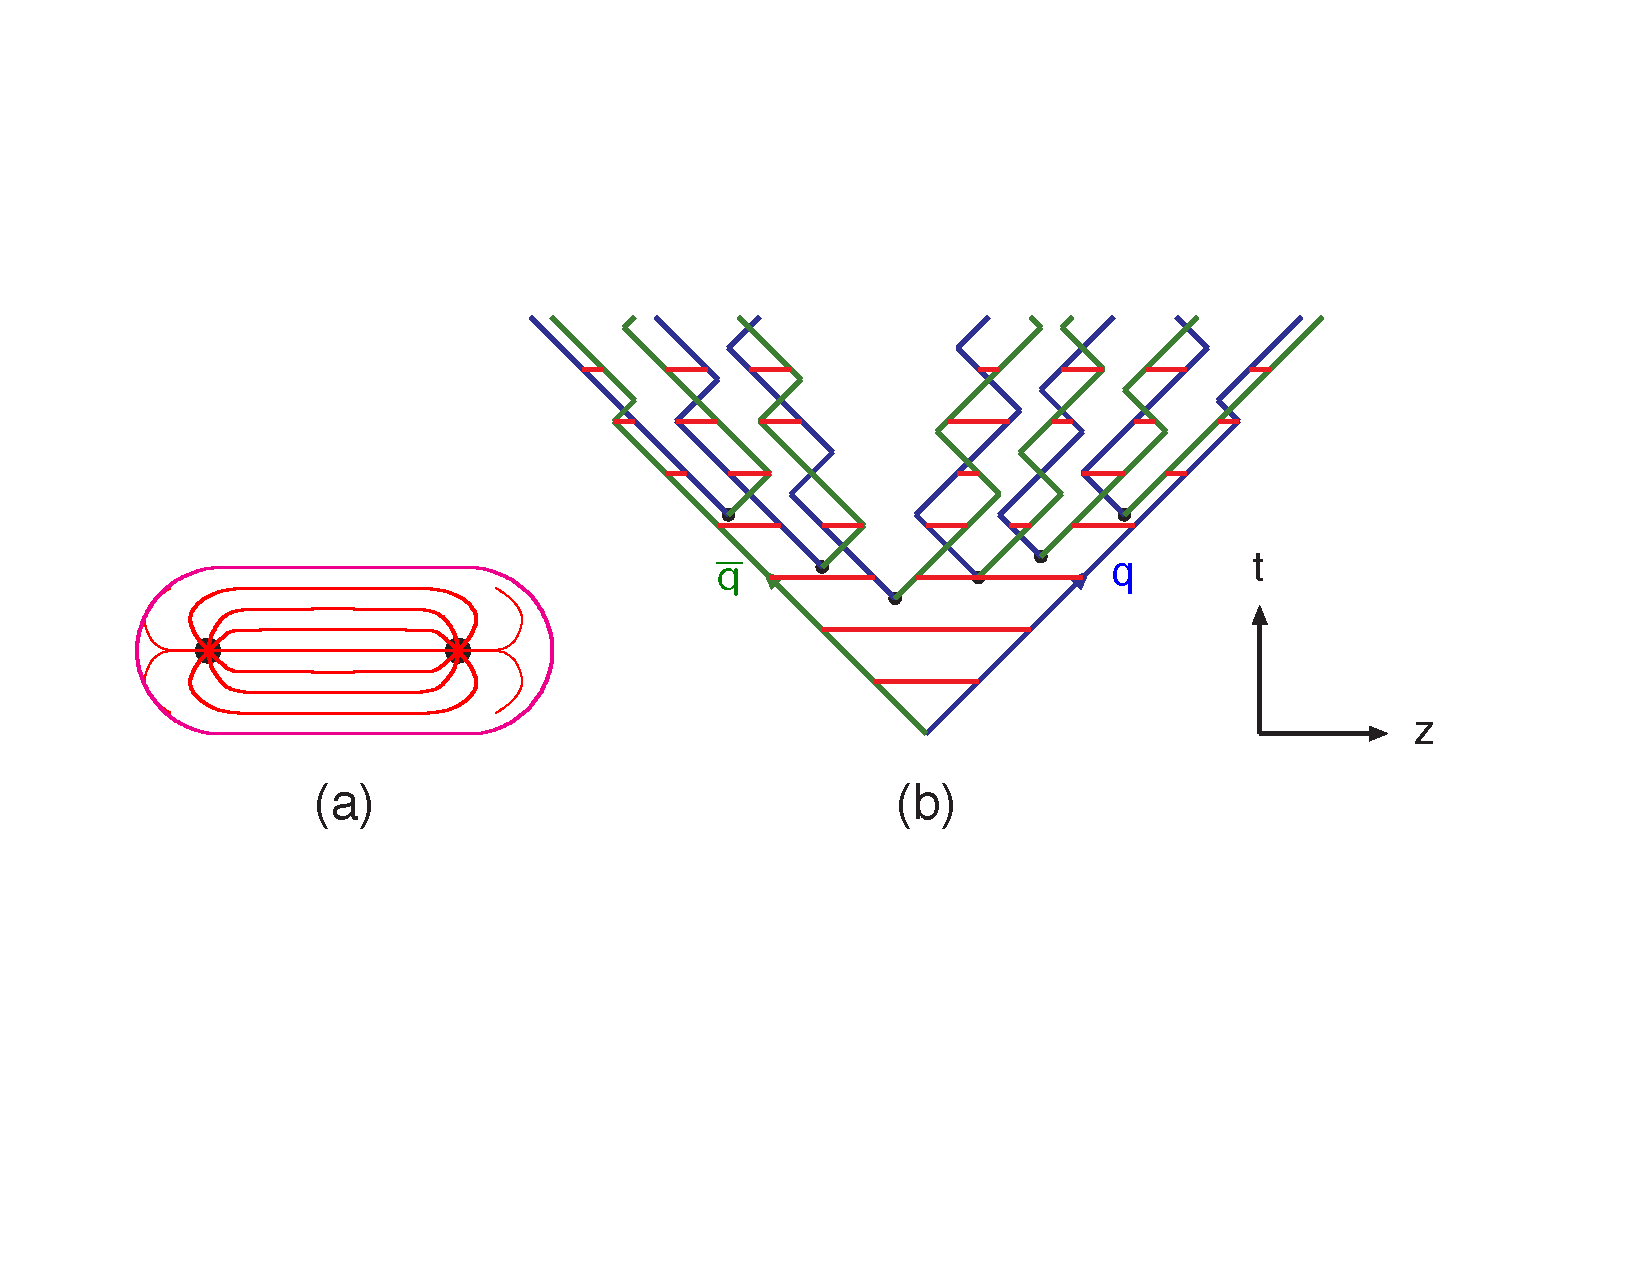
\includegraphics[width=\textwidth]{hadronization/stringone.pdf} 
\caption{(a) A flux tube spanned between a quark and an antiquark.
(b) The motion and breakup of a string system, with the two 
transverse degrees of freedom suppressed (diagonal lines are 
(anti)quarks, horizontal ones snapshots of the string field).
\label{fig:stringone}}
\end{figure}

In QCD, a linear confinement is expected at large distances. This
provides the starting point for the string model, most easily
illustrated for the production of a back-to-back $q\overline{q}$ 
pair, \eg in $e^+e^-$ annihilation events. As the partons move 
apart, the physical picture is that of a colour flux tube being 
stretched between the $q$ and the $\overline{q}$, 
\FigRef[a]{fig:stringone}. The transverse dimensions of the tube 
are of typical hadronic sizes, roughly 1~fm. If the tube is assumed 
to be uniform along its length, this automatically leads to a 
confinement picture with a linearly rising potential, 
$V(r) = \kappa r$. From hadron mass spectroscopy the string 
constant $\kappa$, \ie the amount of energy per unit length, 
is known to be 
$\kappa \approx 1~\mathrm{GeV/fm} \approx 0.2~\mathrm{GeV}^2$.

This picture is also supported by lattice QCD calculations in the 
quenched approximation, \ie with a gluonic field but no dynamical 
quarks. At small distances an additional Coulomb term is required,
but the assumption of the Lund model is that this term can be 
neglected in the overall production pattern of hadrons. Its 
influence would be felt in the properties of the individual  
hadrons, such as wave functions and masses, however.

In order to obtain a Lorentz covariant and causal description of the 
energy flow due to this linear confinement, the most straightforward 
approach is to use the dynamics of the massless relativistic string with 
no transverse degrees of freedom. The mathematical, one-dimensional 
string can be thought of as parameterizing the position of the axis 
of a cylindrically symmetric flux tube.  The expression ``massless'' 
relativistic string is somewhat of a misnomer: $\kappa$ effectively 
corresponds to a ``mass density'' along the string.

Now consider a simple $q\overline{q}$ two-parton event further.
As the $q$ and $\overline{q}$ move apart from the creation vertex, 
say along the $\pm z$ axis, the potential energy stored in the string 
increases, and the string may break by the production of a new 
$q'\overline{q}'$ pair, so that the system splits into two 
colour-singlet systems $q\overline{q}'$ and $q'\overline{q}$. 
These two systems move apart, and a widening no-field region opens up
in between, \FigRef[b]{fig:stringone}. For simplicity the quarks are 
shown as massless, so they move with the speed of light. If the 
invariant mass of either of these systems is large enough, further 
breaks may occur, and so on until only ordinary hadrons remain. 
Typically, a break occurs when the $q$ and the $\overline{q}$ ends 
of a colour singlet system are 1--5~fm apart in the $q\overline{q}$ 
rest frame, but note that the higher-momentum particles at the 
outskirts of the system are appreciably Lorentz contracted.

At the end of the process, the string has broken by the creation of a 
set of new $q_i\overline{q}_i$ pairs, with $i$ running from 1 to
$n-1$ for a system that fragments into $n$ primary hadrons (\ie
hadrons before secondary decays). Each hadron is formed by the quark 
from one break (or an endpoint) and the antiquark from an adjacent break:
$q\overline{q}_1$, $q_1\overline{q}_2$, $q_2\overline{q}_3$, \ldots, 
$q_{n-1}\overline{q}$.

The space--time picture of string motion, \eg in 
\FigRef[b]{fig:stringone}, can be mapped onto a corresponding 
energy--momentum picture by noting that the constant string tension 
implies that the quarks obey 
\begin{equation}
\left| \frac{\mathrm{d}E}{\mathrm{d}z} \right| =
\left| \frac{\mathrm{d}p_z}{\mathrm{d}z} \right| = 
\left| \frac{\mathrm{d}E}{\mathrm{d}t} \right| =
\left| \frac{\mathrm{d}p_z}{\mathrm{d}t} \right| = \kappa ~.
\label{eq:stringtension}
\end{equation}
It follows that a hadron formed between vertices $1$ and $2$ has 
$E = \kappa\Delta z = \kappa(z_1 - z_2)$ and 
$p_z = \kappa\Delta t = \kappa(t_1 - t_2)$ 
\cite{Andersson:1983ia}. The different breaks are spacelike separated, 
$(\Delta t)^2 - (\Delta z)^2 < 0$, \ie they occur ``independently'' 
of each other in a causal sense. Nevertheless two adjacent
breaks are constrained by the fact that the string piece created
by them has to be on the mass shell for the hadron being produced:
$m_{\perp}^2 = m^2 + p_x^2 + p_y^2 = E^2 - p_z^2 = %
\kappa^2((\Delta z)^2 - (\Delta t)^2)$,
\FigRef[a]{fig:stringtwo}. Here transverse mass is introduced, since
it is this quantity that becomes relevant for the $(E, p_z)$ and 
$(t, z)$ pictures, rather than normal mass, once transverse momentum 
fluctuations are introduced, see below. The total probability for an 
event to be formed can therefore be written as the product of $n-1$ 
breakup vertex probabilities times $n$ delta functions for the 
(transverse) hadron masses.

\begin{figure}
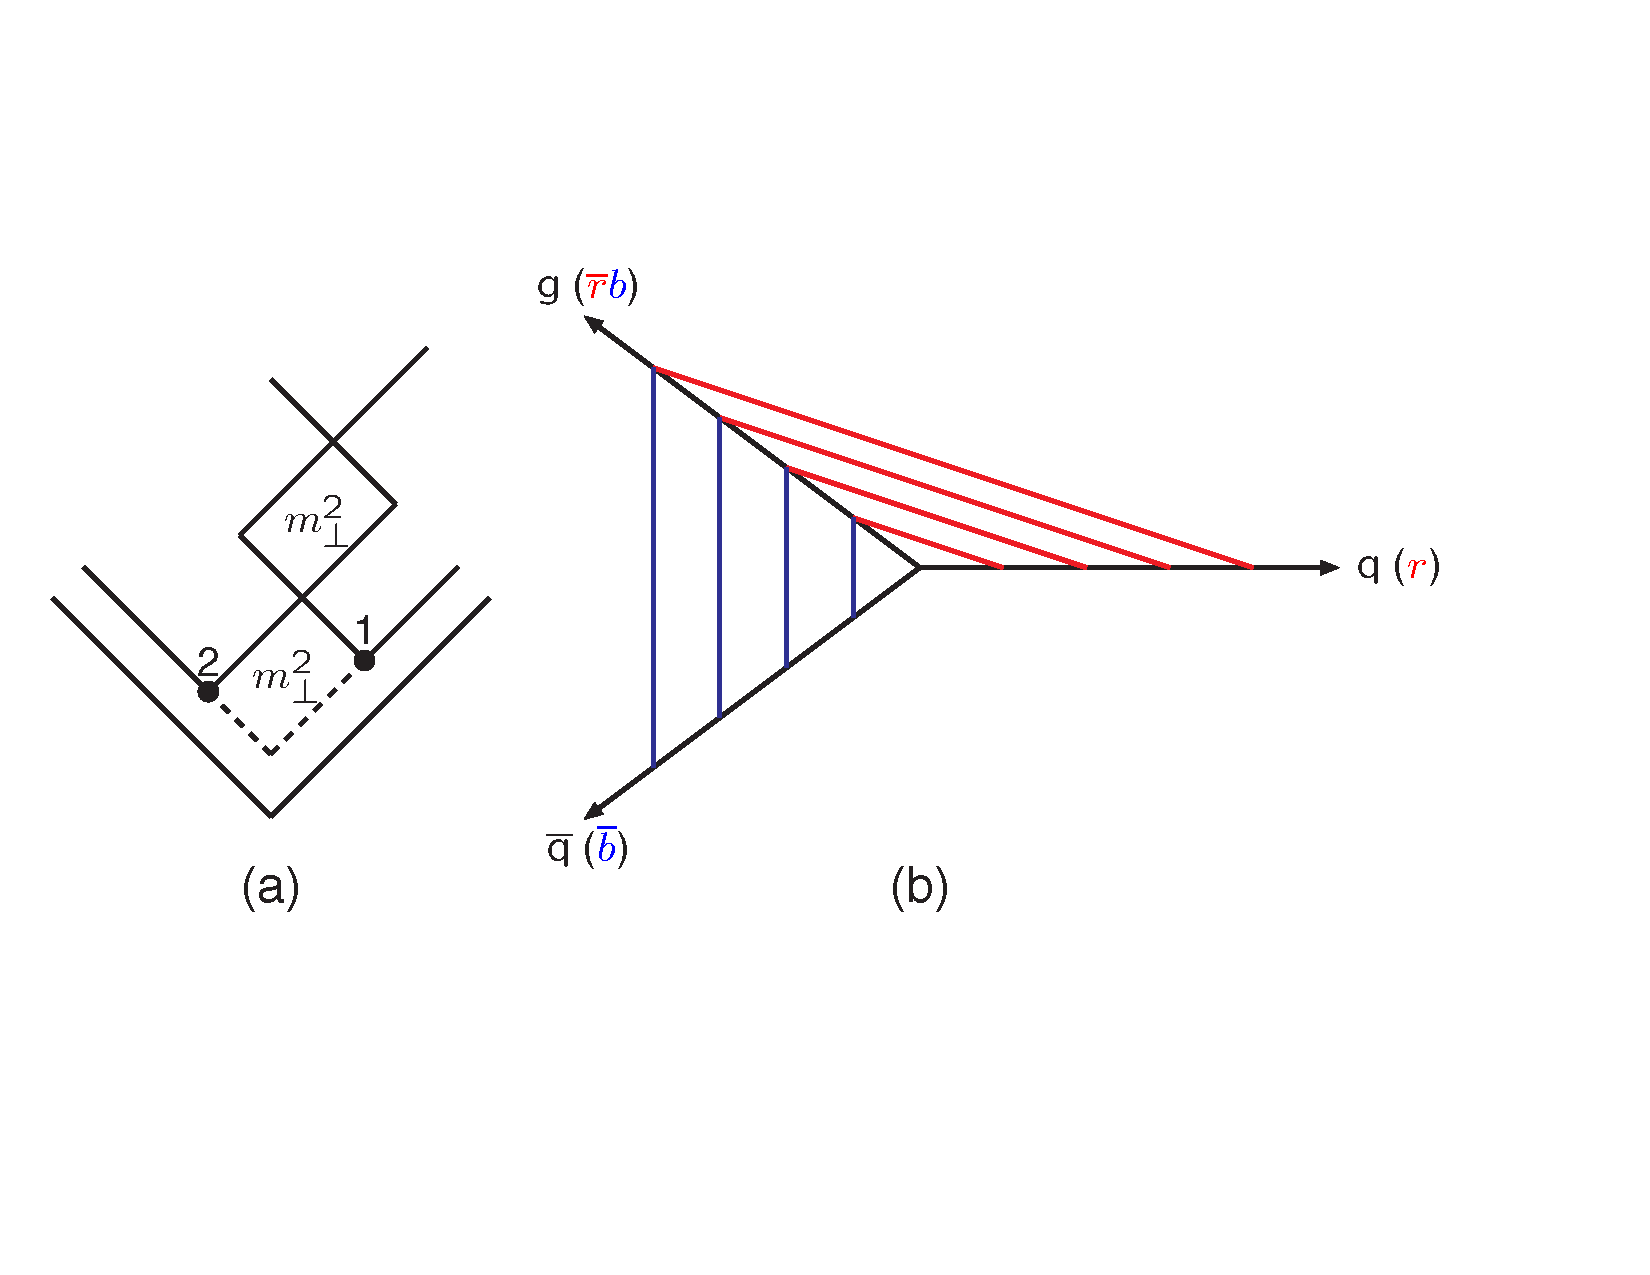
\includegraphics[width=\textwidth]{hadronization/stringtwo.pdf} 
\caption{(a) conditions on nearby string breaks;
(b) string motion in three-jet $q\overline{q}g$ events
\label{fig:stringtwo}}
\end{figure}

Technically such an approach would be cumbersome. Fortunately 
an iterative procedure can be used to give the same result.
Since there is no natural ordering, one is free to consider the 
breaks in any order. For instance, one can start
at the $q$ end of the system and iterate ``left'' towards the 
$\overline{q}$ end. Alternatively, one can start at the 
$\overline{q}$ end and iterate the other way, towards ``right''. 
Either approach should give the same overall answer,
``left--right symmetry''. Focusing on the production of a single
hadron between vertices 1 and 2, \FigRef[a]{fig:stringtwo},
the requirement reads $\mathcal{P}(1) \, \mathcal{P}(1 \to 2) =
\mathcal{P}(2) \, \mathcal{P}(2 \to 1)$, where $\mathcal{P}(i)$
is the probability to reach vertex $i$ by iteration from left/right
and $\mathcal{P}(i \to j)$ the probability to take a step from 
vertex $i$ to vertex $j$.  

The solution to this equation can be written in terms of a 
fragmentation function $f(z)$, where $z$ is the fraction of 
the remaining lightcone momentum that the new hadron takes,
with $E \pm p_z$ fraction for iteration to the left/right:
\begin{equation}
f(z) \propto \frac{1}{z} \, (1 - z)^a \, 
\exp\left( - \frac{b m_{\perp}^2}{z} \right) ~,            
\label{eq:stringfz}
\end{equation}
where $a$ and $b$ are two free parameters (for the derivation
see~\cite{Andersson:1983jt}).\footnote{A more complicated
  expression, with different $a$ parameters for different flavours, is
  possible in principle, but only studied for baryon production.} 

As a by-product, the derivation of $f(z)$ also gives the probability 
distribution in invariant time $\tau$ of $q'\overline{q}'$ breakup 
vertices. In terms of $\Gamma = (\kappa\tau)^2$, this distribution is
$\mathrm{d}\mathcal{P}/\mathrm{d}\Gamma \propto  \Gamma^a \exp(-b \Gamma)$,
with the same $a$ and $b$ as above. In a given event, the connection 
between adjacent $\Gamma$ values is given by the formula
\begin{equation}
\Gamma_2 = (1 - z) \, \left( \Gamma_1 + \frac{m_{\perp}^2}{z} \right) ~, 
\label{eq:stringgamma}
\end{equation}
where $\Gamma_1$ is the ``old'' and $\Gamma_2$ is the ``new'' value 
obtained after taking a step $z$ for the production of a hadron 
with transverse mass $m_{\perp}$. The initial values at the $q$ and 
$\overline{q}$ ends of the system are $\Gamma_0 = 0$. Note that
$a = 0$ corresponds to a pure exponential decay as a function of 
the area swept out by the string, exactly as in the Artru--Mennessier 
model, but that correlations between adjacent $\Gamma_i$ values is  
affected by the difference in mass spectra between the Lund and 
Artru--Mennessier models. 

Heavy quarks, \ie charm and bottom, are not produced at new string 
breaks (see below), but may be at the endpoints of a string. 
Unlike massless quarks, heavy quarks
do not move along straight lines, which implies a
changed area swept out by the string field. The argument of an 
exponential decay with area then leads to a modified shape 
\cite{Bowler:1981sb}
\begin{equation}
f(z) \propto \frac{1}{z^{1 + b m_Q^2}} \, (1 - z)^a \, 
\exp\left( - \frac{b m_{\perp}^2}{z} \right) ~,
\label{eq:stringfzsheavy}
\end{equation}
where $m_Q$ is the heavy-quark mass. 

The $f(z)$ formulae above, for the breakup of a system into a hadron and
a remainder-system, strictly speaking only apply when the mass of the
remainder-system is large. In a Monte Carlo program, it is therefore
necessary to introduce a special procedure to cover the production of
the last two particles. This contains no new physics, but has just to be
constructed so that the place where one selects to ``patch up'' the
fragmentation from the $q$ end with that from the $\overline{q}$ one 
looks as closely like any other as is possible. In addition, steps 
are taken from the left and right ends of the system at random, so that 
the matching procedure is not applied at the same place in all events.

A related but different issue is what to do with a low-mass string,
which occasionally may occur as part of an event with several separate 
strings. An attempt is then made to form an exclusive two-body state, 
with orientation preferentially along the string axis. If the string mass
is too small for this to 
work, there is a possibility to let a small string collapse into one 
single hadron. To put this hadron on the mass shell, some shuffling of 
energy and momentum with other partons in the event is then necessary. 
This machinery thus has some similarities with the cluster fragmentation 
approach, but is in practice only used for a small fraction of the
total particle production.  

In a colour field a $q'\overline{q}'$ pair, where the
$q'$ and $\overline{q}'$ have no mass or transverse momentum, 
can classically be created in one point and then be pulled apart 
by the field. If the quarks have mass or transverse momentum, 
however, they must classically
be produced at a certain distance so that the field energy between
them can be transformed into the transverse mass $m_{\perp}$. Quantum
mechanically, the quarks have to be created in one point and then 
must tunnel out to the classically allowed region. The production 
probability for this tunnelling process is proportional to
\begin{equation}
\exp( -\pi m_{\perp}^2 / \kappa) =  \exp( -\pi m^2 / \kappa) \,
\exp( -\pi p_{\perp}^2 / \kappa) ~.
\label{eq:stringtunnel}
\end{equation}
  
The factorization of the transverse-momentum and the mass terms leads
to a flavour-independent Gaussian spectrum for the 
$q'\overline{q}'$ pairs. Since the string is assumed to have 
no transverse excitations, this $p_{\perp}$ is locally compensated 
between the quark and the antiquark of the pair, and
$\langle p_{\perp q}^2 \rangle = \sigma^2 = \kappa/\pi 
\approx (250~\mathrm{MeV})^2$. Experimentally a number closer to 
$\sigma^2 \approx (350~\mathrm{MeV})^2$
is required, which could be explained as the additional effect of 
soft-gluon radiation below the shower cutoff scale. That radiation 
would have a non-Gaussian shape but, when combined with the ordinary 
fragmentation $p_{\perp}$, the overall shape is close to Gaussian, 
and is parameterized correspondingly in the program. Hadrons receive 
$p_{\perp}$ contributions from two $q'\overline{q}'$ pairs and have 
$\langle p_{\perp h}^2 \rangle = 2 \sigma^2$.
  
The formula also implies a suppression of heavy quark production,
$u : d : s : c \approx 1 : 1 : 0.3 : 10^{-11}$. Charm and heavier quarks
hence are not expected to be produced in the soft fragmentation.
The suppression of $s\overline{s}$ production is left as a free 
parameter in the program, but the experimental value agrees 
qualitatively with theoretical prejudice.
  
A quark and an antiquark may combine to produce either a pseudoscalar
or a vector meson. From counting the number of spin states
one would expect the relative probability for pseudoscalar : vector
to be 1 : 3. This should be modified by wave function effects, as
manifested \eg in the mass splitting between pseudoscalar and vector
mesons, bringing the ratio closer to $1 : 1$. The production of higher 
resonances is assumed to be low in a string framework. The four 
$L = 1$ multiplets are implemented, but are disabled by default, largely
because several states are poorly known and thus may result in a 
worse overall description when included. 
  
The simplest scheme for baryon production is that, in addition to
quark--antiquark pairs, also antidiquark--diquark pairs are occasionally 
produced in the field, in a triplet--antitriplet representation.
Such an assumption does not imply that a diquark should be considered as
a single excitation of an elementary field, only that the soft
chromoelectric field effectively acts on a diquark as if it were a single unit.
Due to the large uncertainty in the definition of diquark masses, the
tunnelling formula cannot be used directly to predict the expected rate of
diquark production. Rather, from data a relative probability for diquark
to quark production is determined to be $qq / q \approx 0.1$. Further
parameters are needed to pin down the rates of individual diquarks, 
again for lack of well-defined diquark masses.

A more general framework for baryon production is the so-called
popcorn model, in which diquarks as such are never produced, but
rather baryons appear from the successive production of several 
$q'\overline{q}'$ pairs. Part of the time, the end result will be 
exactly the same $B\overline{B}$ situation as above, \ie with an 
adjacent baryon $B$ and antibaryon $\overline{B}$ sharing a 
diquark--antidiquark pair. However, further possibilities of the type 
$BM\overline{B}$, $BMM\overline{B}$, etc., can occur,
where a varying number of mesons $M$ are produced in between 
the baryon and antibaryon. The $B$ and $\overline{B}$ then have just 
one $q'\overline{q}'$ pair in common, rather than two. In its present 
form, the program generates $B\overline{B}$ and $BM\overline{B}$ 
configurations with roughly equal probability, while $BMM\overline{B}$ 
and even longer meson chains are neglected.

A given quark--diquark pair may combine to produce either a spin $1/2$
(``octet'') or a spin $3/2$ (``decuplet'') baryon. Again higher resonances 
are neglected. A very important constraint is the fact that a baryon is 
a symmetric state of three quarks, neglecting the colour degree of 
freedom. When a diquark and a quark are joined to form a baryon, it is 
therefore necessary to weight the different flavour and spin states 
by the probability that they form a symmetric three-quark system.

So far only the simplest possible system, $q\overline{q}$, has been
considered. If several partons are moving apart from a common origin, 
the details of the string drawing become more complicated. For a 
$q\overline{q}g$ event, a string is stretched from the $q$ end 
via the $g$ to the $\overline{q}$ end, \FigRef[b]{fig:stringtwo}, 
\ie the gluon is an energy- and momentum-carrying kink on the string. 
It is assigned an incoherent sum of one colour charge and one anticolour 
one. 

As a consequence of the gluon having two string pieces attached, the
ratio of gluon/quark string forces becomes 2, a number that can be
compared with the ratio of colour charge Casimir operators, $\Nc/C_F =
2/(1-1/\Nc^2) = 9/4$. In this, as in several other respects, the
string model can therefore be viewed as a variant of QCD where the
number of colours $\Nc$ is not 3 but infinite (\cf\SecRef{sec:large-nc-limit}).

Note that the factor 2 above does not depend on the kinematical 
configuration: a smaller opening angle between two partons corresponds 
to a smaller string length drawn out per unit time, but also to an 
increased transverse velocity of the string piece, which gives an 
exactly compensating boost factor in the energy density per unit 
string length. 

In an event with several gluons, these will still appear as kinks on 
the string between the $q$ and $\overline{q}$ ends. It is also possible 
to have a closed gluon string, \eg in $\Upsilon \to ggg$ decays.

One of the key predictions of the string model is that, in
$q\overline{q}g$ events, the $qg$ and $\overline{q}g$ angular 
regions should receive enhanced particle production, while the 
$q\overline{q}$ one should be depleted. This arises as a consequence
of having fragmenting string pieces boosted into the former two
regions, but not into the latter one. It was confirmed by JADE 
\cite{Bartel:1983ii}, which inspired the Leningrad study of 
perturbative coherence in such events \cite{Azimov:1986sf}. 
It led to the picture of linked dipoles driving a 
perturbative evolution \cite{Gustafson:1986db,Gustafson:1987rq}, 
\SecRef{sec:dipoles}.  

One of the key virtues of the string fragmentation approach is that it
is collinear and infrared safe. That is, the emission of a collinear or 
soft gluon disturbs the overall string motion and fragmentation 
vanishingly little in the small-angle/energy limit 
\cite{Sjostrand:1984ic}. Therefore the choice of lower cutoff scale 
for parton showers is not crucial: letting the shower evolve to 
smaller and smaller scales just adds smaller and smaller wrinkles 
on the string, which still maintains the same overall shape.% 
\footnote{In a generator implementation there are technical 
complications, however, and also an increasing time consumption, 
implying that it does not pay to take things to the extreme.}

\begin{figure}
\hspace*{0.1\textwidth}
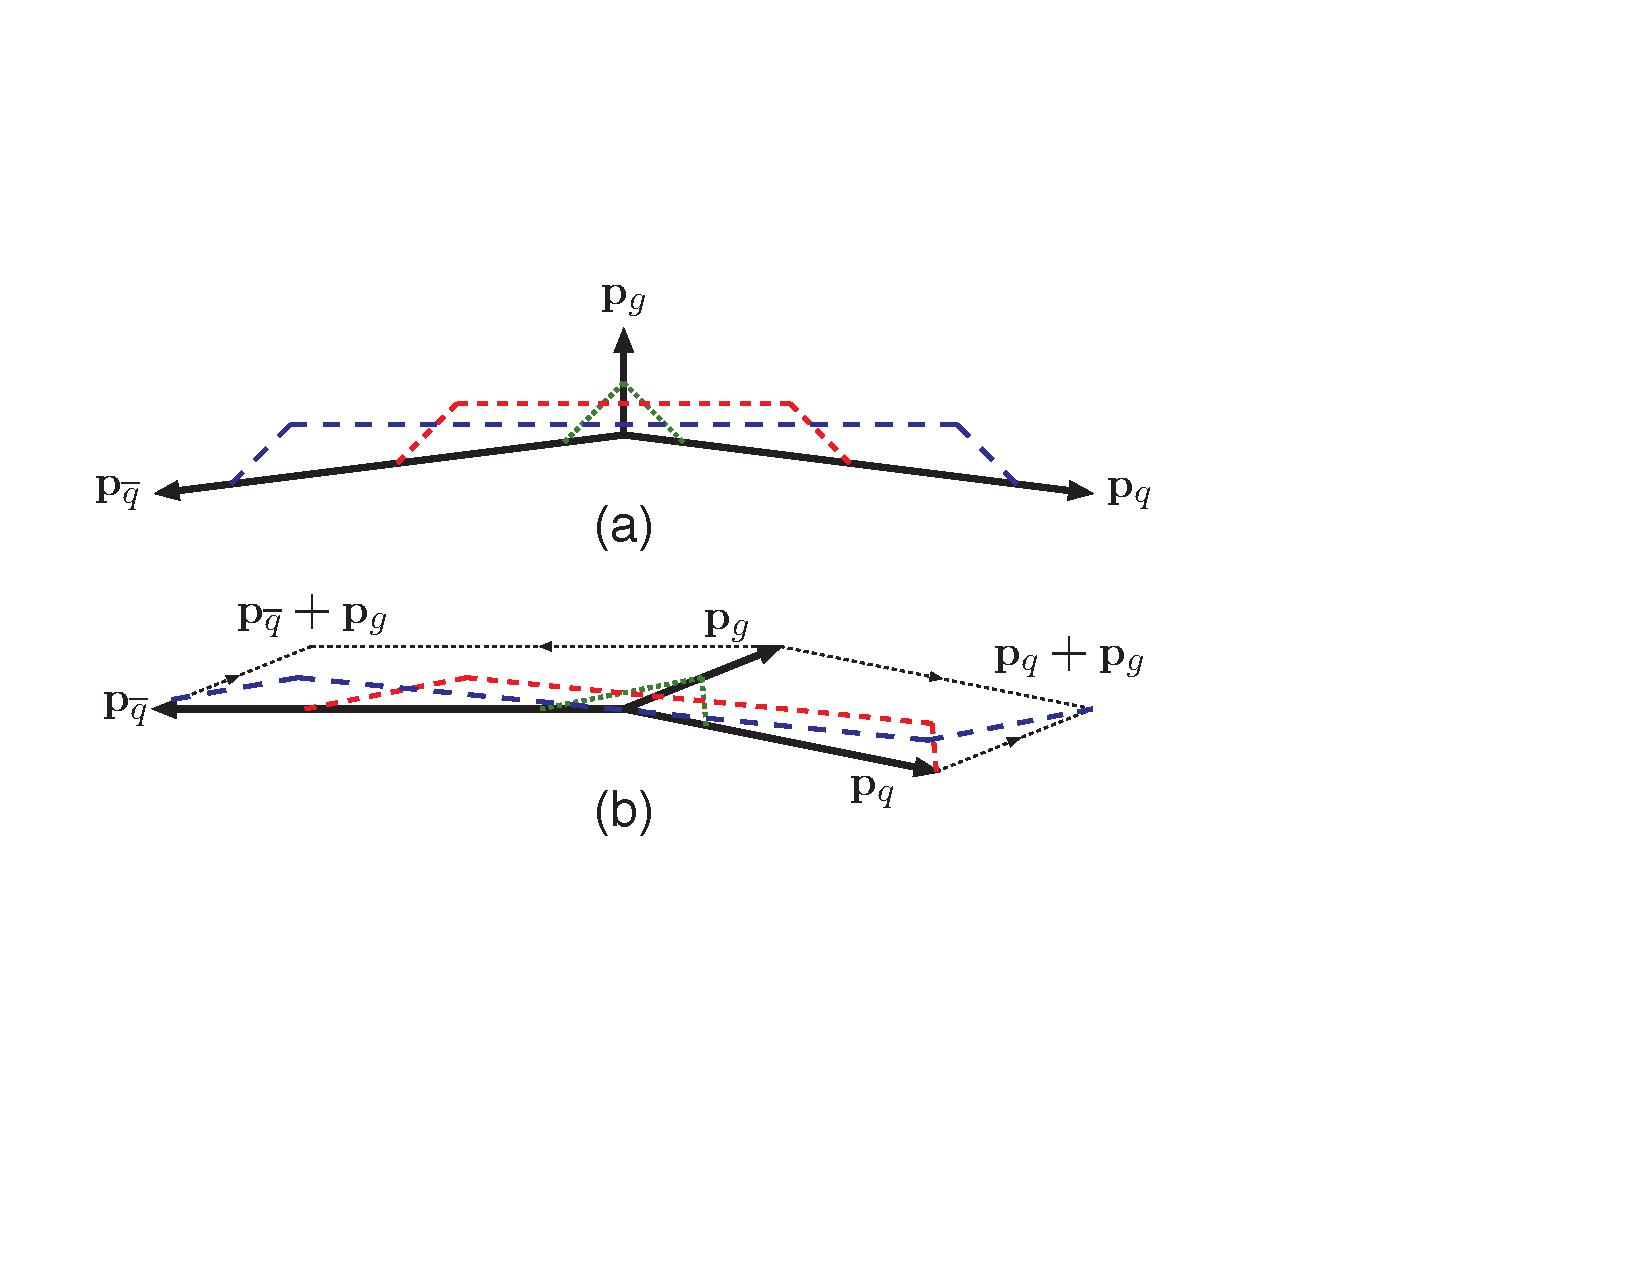
\includegraphics[width=0.8\textwidth]{hadronization/stringthree.pdf} 
\caption{Snapshots in time of the string motion for (a) soft and
(b) collinear gluon emission.
\label{fig:stringthree}}
\end{figure}

To understand this point a bit better, consider the string motion
without any fragmentation. A three-jet $q\overline{q}g$ event initially 
corresponds to having a string stretched from the $q$ via the $g$ to 
the $\overline{q}$, \ie two string pieces, \FigRef[b]{fig:stringtwo}.
In the string piece between the $g$ and the $q$ ($\overline{q}$), 
$g$ four-momentum is flowing towards the $q$ ($\overline{q}$) end,
and $q$ ($\overline{q}$) four-momentum towards the $g$ end. When 
the $g$ has lost all its energy, the $g$ four-momentum continues 
moving away from the middle, \ie where the $g$ used to be, and 
instead a third string region is formed there, consisting of inflowing 
$q$ and $\overline{q}$ four-momentum.
  
For an energetic gluon it takes a long time for the gluon to lose its
energy, and by then hadronization is already well under way. For a 
low-energy gluon, on the other hand, the third string region 
appears early, and the overall drawing of the string becomes fairly 
two-jetlike, \FigRef[a]{fig:stringthree}. In the limit of vanishing 
gluon energy, the two initial string regions disappear, and 
the ordinary two-jet event is recovered. Also for a collinear gluon, 
\ie $\theta_{qg}$ (or $\theta_{\overline{q}g}$) small, the stretching 
becomes two-jetlike, \FigRef[b]{fig:stringthree}. In particular, the 
$q$ string endpoint first moves out a distance $\mathbf{p}_q / \kappa$, 
and then a further distance $\mathbf{p}_g / \kappa$, a first half 
accreting gluon four-momentum and a second half re-emitting it.
The end result is, approximately, that a string is drawn out as if
there had only been a single parton with energy 
$|\mathbf{p}_q + \mathbf{p}_g|$, such that the simple two-jet event 
again is recovered in the limit $\theta_{qg} \to 0$.
These discussions for the three-jet case can be extended to the 
motion of a string with an arbitrary number of intermediate gluons. 
  
The generalization of the left--right symmetry requirement to the
fragmentation of multiparton configurations is not completely unique. 
A sensible physics ansatz is that the distribution in 
invariant time of breakup vertices should not depend on the exact 
shape of the string. The $z$ variable no longer has any simple physical 
interpretation, but \EqRef{eq:stringfz} and 
\EqRef{eq:stringgamma} taken together still provide a valid recipe 
for the relationship between adjacent $\Gamma$ values. These $\Gamma$ 
values themselves are always well defined and, if taken together with
the constraint of hadrons being on mass shell, uniquely define the 
position of each breakup vertex.

Until now only the string model as such has been introduced. It is 
useful to briefly put it into the context of the generation of a 
complete event in hadronic collisions, a topic discussed in 
\SecRef{sec:mbmpi-np}. String fragmentation is almost at the end of the
generation chain, only followed by particle decays. It is applied when
a number of partons have already been produced,
by a combination of hard processes and parton showers, and with
coloured leftover beam remnants. Since a remnant cannot be described 
by perturbative means, special rules are needed to assign colours to 
the individual partons in it, and to describe how the available 
remnant momentum is split between them. Some of these rules are 
based on common sense, such as that the average valence quark ought to 
carry more momentum than the sea one, but our ignorance also leads to 
some arbitrary decisions. With the remnant subdivided, and with colours 
traced in the large-$\Nc$ limit, the string topology can be constructed. 
The event that way can be split into a number of string systems. 
Mainly these will be open strings, with quarks or diquarks at the 
endpoints and with gluons in between, but closed gluon loops are 
also possible. 

One special issue is that of baryon number flow if, say, (the colour 
of) two of the valence quarks of a proton are kicked out in different 
directions. For situations like these a three-quark system can be 
viewed as a Y-shaped topology: three strings, each with a quark at 
one endpoint, and at the other coming together in a junction. 
Each of the strings can break by the production of new 
$q'\overline{q}'$ pairs, but at the end of the process there will be one
unmatched $q'$ nearest to the junction in each string, and these 
three together give a baryon. Thus the baryon number is ``carried''
by the junction, and the balance between the different string pieces
pulling on the junction largely determines the net motion of this
baryon \cite{Sjostrand:2002ip}. Depending on the overall colour 
topology of an event it thereby becomes possible to transport 
the baryon number over large rapidity distances.

One potential weakness of the string model is that it is formulated
in terms of the fragmentation of one single string in isolation,
as you may expect it to be in $e^+e^-$ annihilation events. 
If several strings are produced, they fragment independently of each 
other. For hadronic collisions the MPI framework is likely to lead to 
a picture where several strings overlap in space and time during the 
fragmentation process, however, especially at high collision energies. 
It is not unthinkable that this leads to collective phenomena bordering 
on those of the quark--gluon plasma expected in heavy-ion collisions, 
which then are not modelled by the standard string framework. 
For instance, a dense hadronic gas could lead to non-negligible
rescattering corrections.

Finally, in addition to the basic ideas presented here, the string 
concept has been used as a starting point for various extensions, 
say for colour reconnections in $W^+W^-$ events (see
\SecRef{sec:mbmpi-np}) or Bose--Einstein effects among identical
mesons. Such effects are not included in simulations by default.


\mcsubsection{Cluster model}
\label{sec:cluster-model}
The cluster model of hadronization is based on the so-called
preconfinement property of parton showers, discovered by Amati and
Veneziano~\cite{Amati:1979fg}.  They showed that the colour structure of the
shower at any evolution scale $Q_0$ is such that colour singlet
combinations of partons (clusters) can be formed with an
asymptotically universal invariant mass distribution.  Here
`universal' means dependent only on $Q_0$ and the QCD scale $\Lambda$,
and not on the scale $Q$ or nature of the hard process initiating the
shower, while `asymptotically' means $Q\gg Q_0$.  If in addition
$Q_0\gg\Lambda$, then the mass distribution of these colour singlet
clusters, together with their ($Q$-dependent) momentum and
multiplicity distributions, can be computed
perturbatively~\cite{Amati:1979fg,Bassetto:1979vy}.  It turns out that the mass distribution
is power-suppressed at large masses, the mean cluster
multiplicity $\abr{n}$ rises faster than any positive power of $\ln Q$,
and the asymptotic multiplicity distribution is a universal function
of $n/\abr{n}$ (KNO scaling~\cite{Koba:1972ng}).

The preconfinement mechanism can be seen most simply in the limit
of a large number of colours $\Nc$ (\cf\SecRef{sec:large-nc-limit})\footnote{The proof of preconfinement is
  valid for any value of $\Nc$.   However, as in the string model,
  subleading terms of order $1/\Nc^2$ are neglected in the cluster
hadronization model.}.   To leading order in $\Nc$, the gluons in
the shower can be represented by pairs of colour-anticolour lines
that are connected at vertices (see \FigRef{fig:planar}).  Then each
colour line at the low-scale end of the shower is connected to an
anticolour partner line at the same scale.  In this limit the
colour structure of the shower can be drawn on a plane, such that
these colour-anticolour partners are adjacent.  Adjacent partners can
form colour singlets, whereas non-adjacent lines have a vanishing
probability of doing so as $\Nc\to\infty$.   Furthermore, adjacency
tends to imply closeness in phase space, leading to the suppression of large
masses and an asymptotically universal mass distribution of adjacent
objects.  

\begin{figure}
\begin{center}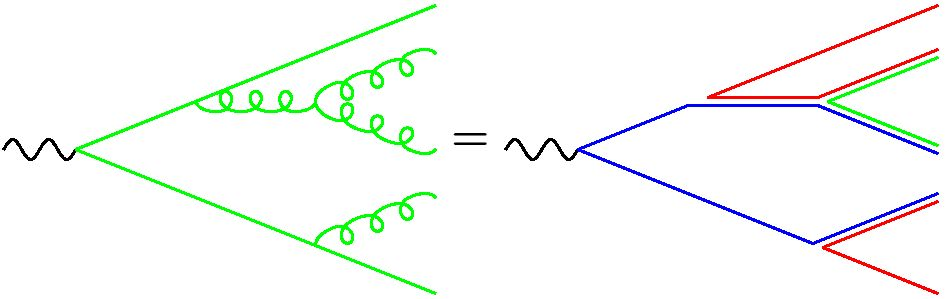
\includegraphics[width=8cm]{hadronization/planar.jpg}\end{center}
\caption{Colour structure of a parton shower to leading order in
  $\Nc$.\label{fig:planar}}
\end{figure}

A model of hadronization based on preconfinement was first proposed by
Wolfram~\cite{Wolfram:1980gg} and incorporated into an event generator for $e^+e^-$
annihilation by Field, Fox and Wolfram~\cite{Fox:1979ag,Field:1982dg}.  The key idea
was to enforce non-perturbative splitting of gluons into
quark-antiquark pairs at the shower cutoff scale $Q_0$.  Then
adjacent colour lines become quark-antiquark pairs that can form
physical clusters with mesonic quantum numbers.  For low values of the
cutoff, the typical cluster invariant masses will be low and the hadrons
from the decay of each cluster will be spread over a limited region of
phase space.  This leads naturally to a distribution of final-state
hadrons closely connected to that of partons at the cutoff scale,
\ie to local parton-hadron duality~\cite{Azimov:1984np,Azimov:1985by}.

The enforced gluon splitting corresponds to an effective enhancement
of the $g\to q\bar q$ vertex, which would be expected to reduce or
even reverse the running of the QCD coupling at low scales.  Thus this
mechanism also agrees, at least qualitatively, with the notion of a finite
effective low-scale value of $\alpha_S$, which is suggested by studies
of hadronization corrections to event shapes\cite{Dokshitzer:1995zt,Dokshitzer:1995qm,Dasgupta:2003iq}
 and jet profiles~\cite{Dasgupta:2007wa}.
 
Another intriguing hint of enhanced gluon splitting is the high
yield of soft photons in hadronic $Z^0$ decays~\cite{Abdallah:2005wn,Abdallah:2010tk}, which cannot be
explained in terms of radiation from perturbatively produced quarks
plus bremsstrahlung from initial-state leptons and final-state hadrons.
This suggests a nonperturbative phase in which many charged particles
are formed and propagate for significant times before hadronization,
as might happen between gluon splitting and cluster formation.

Once the mechanism of gluon splitting has been adopted, a number of
issues need to be addressed in building a quantitative model of
hadronization.  First of all, what should be the momentum distribution
and flavours of the quarks produced in gluon splitting?  The
momentum distribution is not a major issue as long as the
light flavours are treated as having constituent quark masses, $m_{u,d}\sim
300$~MeV, $m_s\sim 450$~MeV.  Then the effective gluon mass at the end
of showering, $m_g\sim Q_0\sim 1$~GeV, is close to the threshold for splitting,
and the kinematic range of quark momentum is too small for it to have 
much effect on the momenta and masses of the clusters.

On the other hand the flavour distribution in gluon splitting will clearly
be important.  At such low scales, kinematics will ensure that heavy flavours are
forbidden and strangeness suppressed.   However, these flavours can be
pair-produced in cluster decays, as can baryon-antibaryon pairs.
Baryons might also come from gluon splitting into light
diquark-antidiquark pairs. Parameters can be introduced to tune the
yields of different flavours, but generally the effects of kinematics
work quite well as a first approximation. 

The cluster mass distribution in $e^+e^-$ annihilation into
light-quark pairs, obtained from the \Herwig\ event generator, is shown in
\FigRef{fig:cluster} for a wide range of  centre-of-mass energies.
One sees clearly the universality of the distribution and the typically
low scale of cluster masses, determined by the shower cutoff,  $Q_0\sim 1$~GeV.

\begin{figure}
\begin{center}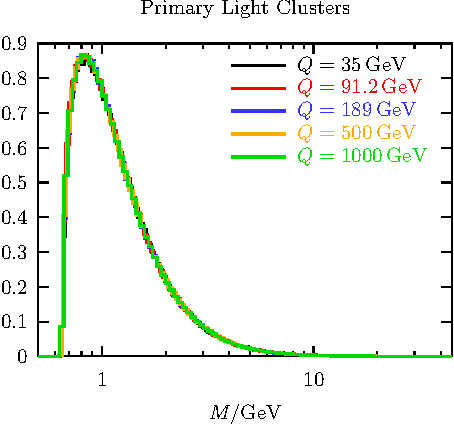
\includegraphics[width=8cm]{hadronization/cluster_mass.pdf}\end{center}
\caption{Invariant mass distribution of colour-singlet clusters in \herwig.\label{fig:cluster}}
\end{figure}

Once these clusters have been formed, how should they decay into the
observed hadrons?  The typical cluster masses are low enough for them
to be treated as a smoothed-out spectrum of excited mesons, in which
case quasi-two-body decay into less excited states seems to be
preferred by Nature.   Assuming that matrix element effects tend to average out,
the simplest model is then to select at random among all two-body decay
channels allowed by flavour and kinematics, with probabilities
proportional to the available phase space for each, including spin
degeneracy.  The preference for decay directly to the lowest-mass
states is somewhat offset by the larger number of spin states amongst
excited hadrons.  One must be careful to include full flavour
multiplets of hadrons of each spin and parity, in order not to bias
the flavour selection. This can entail some guesswork about the masses
and decays of excited heavy-flavour hadrons that are not yet well established.

This basic model of cluster decay comes surprisingly
close to fitting the hadron distributions observed in jet
fragmentation, with virtually no free parameters other than the shower
cutoff.  The multiplicities of different flavours of mesons and
baryons are determined by their masses and spins, and their
transverse momenta relative to the jet axis are naturally limited by
the phase space available in cluster decay. The characteristic
differences between quark and gluon jets, with the latter having
softer hadron spectra, higher multiplicities and wider profiles, all come
from the higher rate of parton showering from gluons; apart from
leading flavour effects, the relative proportions of different hadron species
in all types of jets should be universal.

For a more refined description of hadronic final states, at the level
demanded nowadays from event generators, the basic cluster model
described above requires some adjustments.  The sharp
transition from perturbative to non-perturbative physics at the
cutoff scale tends to over-suppress heavy states such as
multiply-strange (\eg $\Omega^-$) and charmed baryons.  A smoother
transition over a range of scales would clearly be more physical.
Light-flavour baryon production
comes mainly from the decay of mesonic clusters into baryon-antibaryon
pairs.   While this gives about the right multiplicities, it tends to
produce pairs that are too closely correlated in rapidity.  The
requirement that each cluster should produce at least two hadrons leads
to single-hadron distributions that are too low at high fractions of the
jet momentum.  This can be improved somewhat by allowing low-mass
clusters to form a single hadron, transferring some four-momentum
to a `nearby' cluster.  In reality the parton showering mechanism
is not dominant at very high momentum fractions and more exclusive
processes must take over.

 A related problem is the treatment of
high-mass clusters.  Although the cluster mass distribution is
mostly confined to low values, there is always a high-mass tail, as
seen in \FigRef{fig:cluster}, coming from events with very little
parton showering.   Again, exclusive hadron production
would in fact predominate over these highly Sudakov-suppressed
parton configurations.  In the absence of such contributions, special
treatment of high-mass clusters is required, as  the model of
isotropic phase-space decay is clearly unreasonable.  The prescription
commonly adopted is sequential binary fission, preserving the
orientation along the axis defined by the constituent partons of the
original cluster, until the sub-cluster masses fall below some value,
typically  $3-4$~GeV, after which the standard phase-space decay is
resumed.  The treatment of high-mass clusters thus becomes close to
that of the string model, and indeed a smooth merging of the two
models at intermediate cluster masses would seem well worth investigation. 

The two cluster hadronization models in wide
use~\cite{Webber:1983if,Winter:2003tt},
incorporated in the \Herwig\ and \Sherpa\ generators respectively, differ in
their detailed treatment of these issues but follow the basic approach
outlined above.  The reader is referred to the papers cited, the relevant sections
below, and the generator manuals for further details.

An interesting recent development is the application of a statistical
hadronization model to cluster decay~\cite{Bignamini:2010jy}.  In this
way one may generate the spectra, multiplicities and flavour
composition of the produced hadrons with few free parameters, while
retaining the limited transverse momenta and jet structure which are
difficult to explain if a statistical approach is applied directly to the whole
final state.

As in the case of the string model, the basic cluster model does
not include interaction between clusters, except for some
momentum transfer to permit light ones to form single hadrons.
There are optional schemes for colour reconnection between clusters,
for example in $W^+W^-$ hadronic decays, as discussed in
\SecRef{sec:mbmpi-np}.  There could be additional collective effects
when the cluster density becomes high.

\mcsubsection{Summary}
\begin{itemize}
\item Hadronization cannot be calculated from first principles, but has
  to be modelled. The two most commonly used model classes are the string
  and cluster ones. 
\item The string model is based on the assumption of linear confinement.
\item A quark corresponds to an endpoint of a string, and a gluon to a
  kink on it, with partons ordered in colour along the string.
\item The string offers a very predictive framework for how its 
  space--time motion and breakup translates into an energy--momentum
  distribution of the primary hadrons. 
  This framework also applies for complicated multiparton 
  configurations, and has been successfully tested in $e^+e^-$ collisions.
\item The main (known) weakness of the string model is that there are 
  many parameters related to flavour properties, which ultimately have 
  to be pinned down from data itself.
\item The cluster hadronization model is based on the preconfinement
  property of parton showers, which leads to colour-singlet parton
  clusters with a universal mass distribution at low scales.
\item Cluster hadronization starts with non-perturbative splitting of
  gluons into quark-antiquark (and possibly diquark-antidiquark) pairs.
  Clusters are then formed from colour-connected pairs. 
\item Most clusters undergo quasi-two-body sequential phase-space
  decay.  The limited cluster mass spectrum naturally leads to limited
  transverse momenta and suppression of heavy flavour, strangeness and
  baryon production.
\item The decay of heavier clusters requires a more string-like
  initial stage of anisotropic decay into lighter clusters.
\item When combined with angular-ordered parton showers, the cluster
  model gives a fairly good overall description of high-energy
  collider data, usually slightly less good than the string model but
  with fewer parameters.
\item The busy environment of high-energy hadronic collisions could lead to
  nontrivial collective effects, currently not simulated either in string
  or in cluster models. 
\end{itemize}


% Local Variables: 
% mode: LaTeX
% TeX-master: "../mcreview"
% End: 
